\documentclass[]{article}
\usepackage[a4paper, total={6in, 10in}]{geometry}
\usepackage{hyperref}
\usepackage{amsmath}
\usepackage{graphicx}
\usepackage[outdir=./]{epstopdf}
\usepackage{booktabs}
\usepackage{float}
\usepackage{subcaption}

\setlength{\parindent}{0em}
\setlength{\parskip}{1em}

\DeclareMathOperator{\cov}{cov}

%opening
\title{SSY 230, System Identification\\
	Project 1: Estimating functions from noisy data}
\author{Yuxuan Xia\\ \href{mailto:yuxuan.xia@chalmers.se}{yuxuan.xia@chalmers.se}\\Emil Staf\\\href{mailto:emil.staf@chalmers.se}{emil.staf@chalmers.se}}

\begin{document}

\maketitle

\section{ARX estimator}
\subsection{(a) arxfit}
The \emph{arxfit} fucntion can beneficially be implemented using the Linear Regression code written in project 1. The ARX model is given by
\begin{align}
	\label{eq:ARX}
	A(q^{-1})y(t) &= B(q^{-1})u(t) + e(t) \\
	\theta &= (a_1, \ldots a_{na}, b_1, \ldots, b_{nb})^\mathsf{T}
\end{align}
according to (6.13a) in S \& S. This can be rewritten on a Linear Regression format
\begin{equation}
	\label{eq:ARX_LR}
	y(t) = \phi(t) \theta + e(t)
\end{equation}
where
\begin{equation}
	\label{eq:ARX_LR_phi}
	\phi(t) = (-y(t-1), \ldots, -y(t-na), u(t-1-nk), \ldots, u(t-1-nk-nb))^\mathsf{T}
\end{equation}
The function arxfit is implemented accordingly. It was verified against the function 
\begin{equation}
	\label{eq:system}
	y(t) = 0.2y(t-1) - 0.3y(t-2) + 0.4u(t-2) - 0.2u(t-3)
\end{equation}
without any noise, and the correct model was obtained.

\subsection{(b) id2tf}
The function \emph{id2tf} is implemented using MATLABs build in function \emph{tf(Numerator, Denominator, -1)} where \emph{Numerator} = $(\hat{b}_1, \ldots, \hat{b}_{nb})$ and \emph{Denominator} = $(1, \hat{a}_1, \ldots, \hat{a}_{na})$.

\begin{figure}[ht]
\centering
\begin{subfigure}{.49\textwidth}
	\centering
	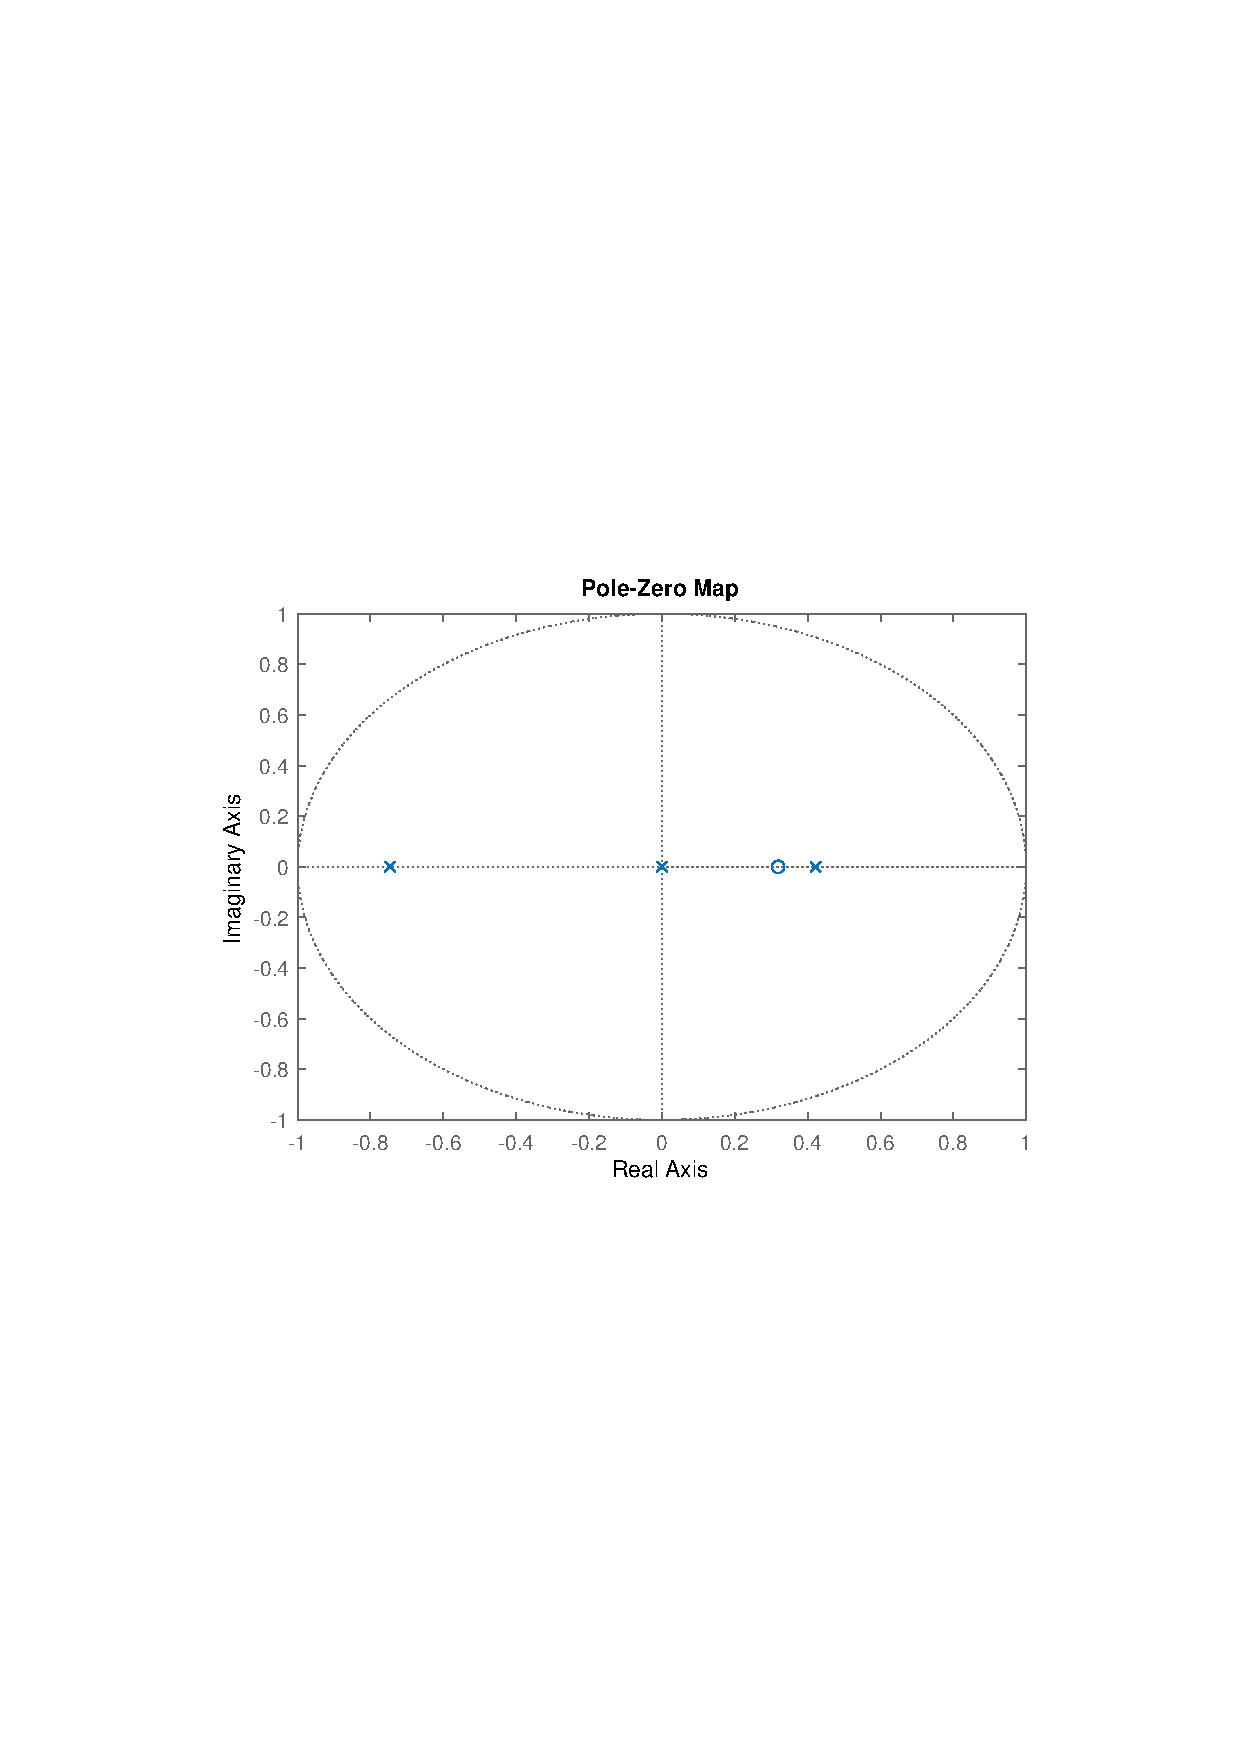
\includegraphics[trim= 10cm 8cm 10cm 8cm, scale=0.4]{figures/1b-pzmap.pdf}
	\caption{pzmap using ltiview}
	\label{fig:1b-pzmap}
\end{subfigure}
\begin{subfigure}{.49\textwidth}
	\centering
	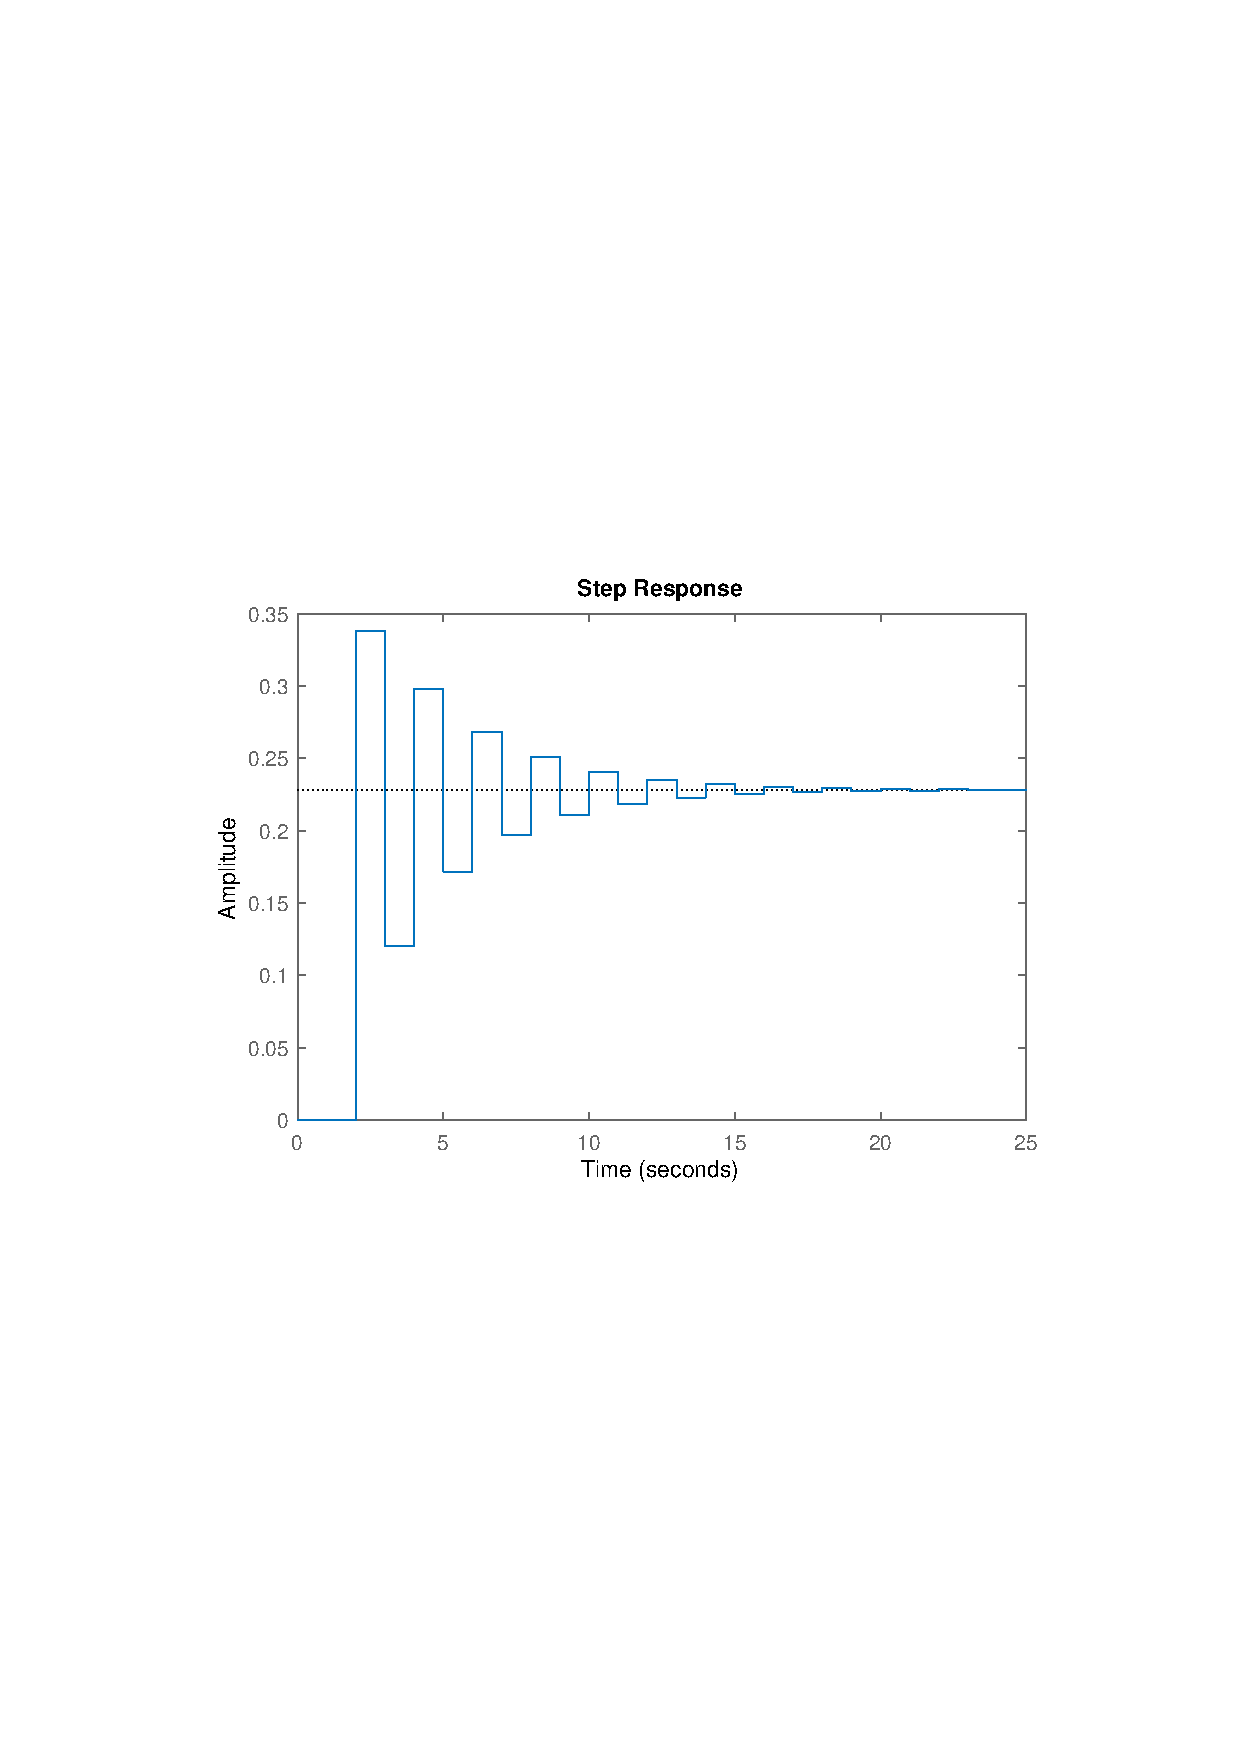
\includegraphics[trim= 10cm 8cm 10cm 8cm, scale=0.4]{figures/1b-step.pdf}
	\caption{Step response using ltiview}
	\label{fig:1b-step}
\end{subfigure}
\caption{MATLABs build in function \emph{ltiview} analyzing the found ARX model for the system in \eqref{eq:system} including noise.}
\label{fig:1b-ltiview}
\end{figure}

\subsection{(c) idpredict and idsimulate}
A $k$-step predictor for an ARX model can be fund by studying the following equations.
\begin{align}
	\label{eq:K-step predictor}
	\hat{y}(t|t-1) &= -a_1y(t-1) -a_2y(t-2) \ldots \\
	\hat{y}(t|t-2) &= -a_1\hat{y}(t-1|t-2) -a_2y(t-2) \ldots \\
	\hat{y}(t|t-3) &= -a_1\hat{y}(t-1|t-3) -a_2\hat{y}(t-2|t-3) \ldots 
\end{align}
It is possible to use the 1-step ahead predictor to calculate the 2-step predictor, the 1-step and 2-step predictor to calculate the 3-step predictor and so on. It is the regressor matrix $\Phi_i = [Y_i, U]$ that needs to be updated in a clever way in order to achieve fast matrix calculations which is shown below. The $U$ matrix is constant and given by

\begin{equation}
	U = \begin{bmatrix}
		u(0-n_k) & u(-1-n_k) & \ldots & u(1-n_b-n_k) \\
		u(1-n_k) & u(0-n_k) & \ldots & u(2-n_b-n_k) \\
		u(2-n_k) & u(1-n_k) & \ldots & u(3-n_b-n_k) \\
		\vdots & \vdots & \vdots & \vdots \\
		u(n-1-n_k) & u(n-2-n_k) & \ldots & u(n-n_b-n_k) \\
	\end{bmatrix}
\end{equation}
while
\begin{equation}
	Y_1 = \begin{bmatrix}
		y(0) & y(-1) & \ldots & y(1-n_a) \\
		y(1) & y(0) &\ldots & y(2-n_a) \\
		y(2) & y(1) &\ldots & y(3-n_a) \\
		\vdots & \vdots & \vdots & \vdots \\
		y(n-1) & y(n-2) & \ldots & y(n-n_a) \\
	\end{bmatrix}
\end{equation}
\begin{equation}
	Y_2 = \begin{bmatrix}
		\hat{y}(0|-1) & y(-1) & \ldots & y(1-n_a) \\
		\hat{y}(1|0) & y(0) &\ldots & y(2-n_a) \\
		\hat{y}(2|1) & y(1) &\ldots & y(3-n_a) \\
		\vdots & \vdots & \vdots & \vdots \\
		\hat{y}(n-1|n-2) & y(n-2) & \ldots & y(n-n_a) \\
	\end{bmatrix}
\end{equation}
\begin{equation}
Y_3 = \begin{bmatrix}
		\hat{y}(0|-2) & \hat{y}(-1|-2) & \ldots & y(1-n_a) \\
		\hat{y}(1|-1) & \hat{y}(0|-1) &\ldots & y(2-n_a) \\
		\hat{y}(2|0) & \hat{y}(1|0) &\ldots & y(3-n_a) \\
		\vdots & \vdots & \vdots & \vdots \\
		\hat{y}(n-1|n-3) & \hat{y}(n-2|n-1) & \ldots & y(n-n_a) \\
	\end{bmatrix}
\end{equation}
where $\hat{y}(t|t-k) = \Phi_k \hat{\theta}$ and the values for both $y$ and $u$ prior to $t=1$ are initialized to zero.

\subsection{(d) idcompare}
Some results for the same system as before \eqref{eq:system} are compared using \emph{idcompare} in Figure \ref{fig:1d}.
\begin{figure}[ht]
\centering
\begin{subfigure}{.30\textwidth}
	\centering
	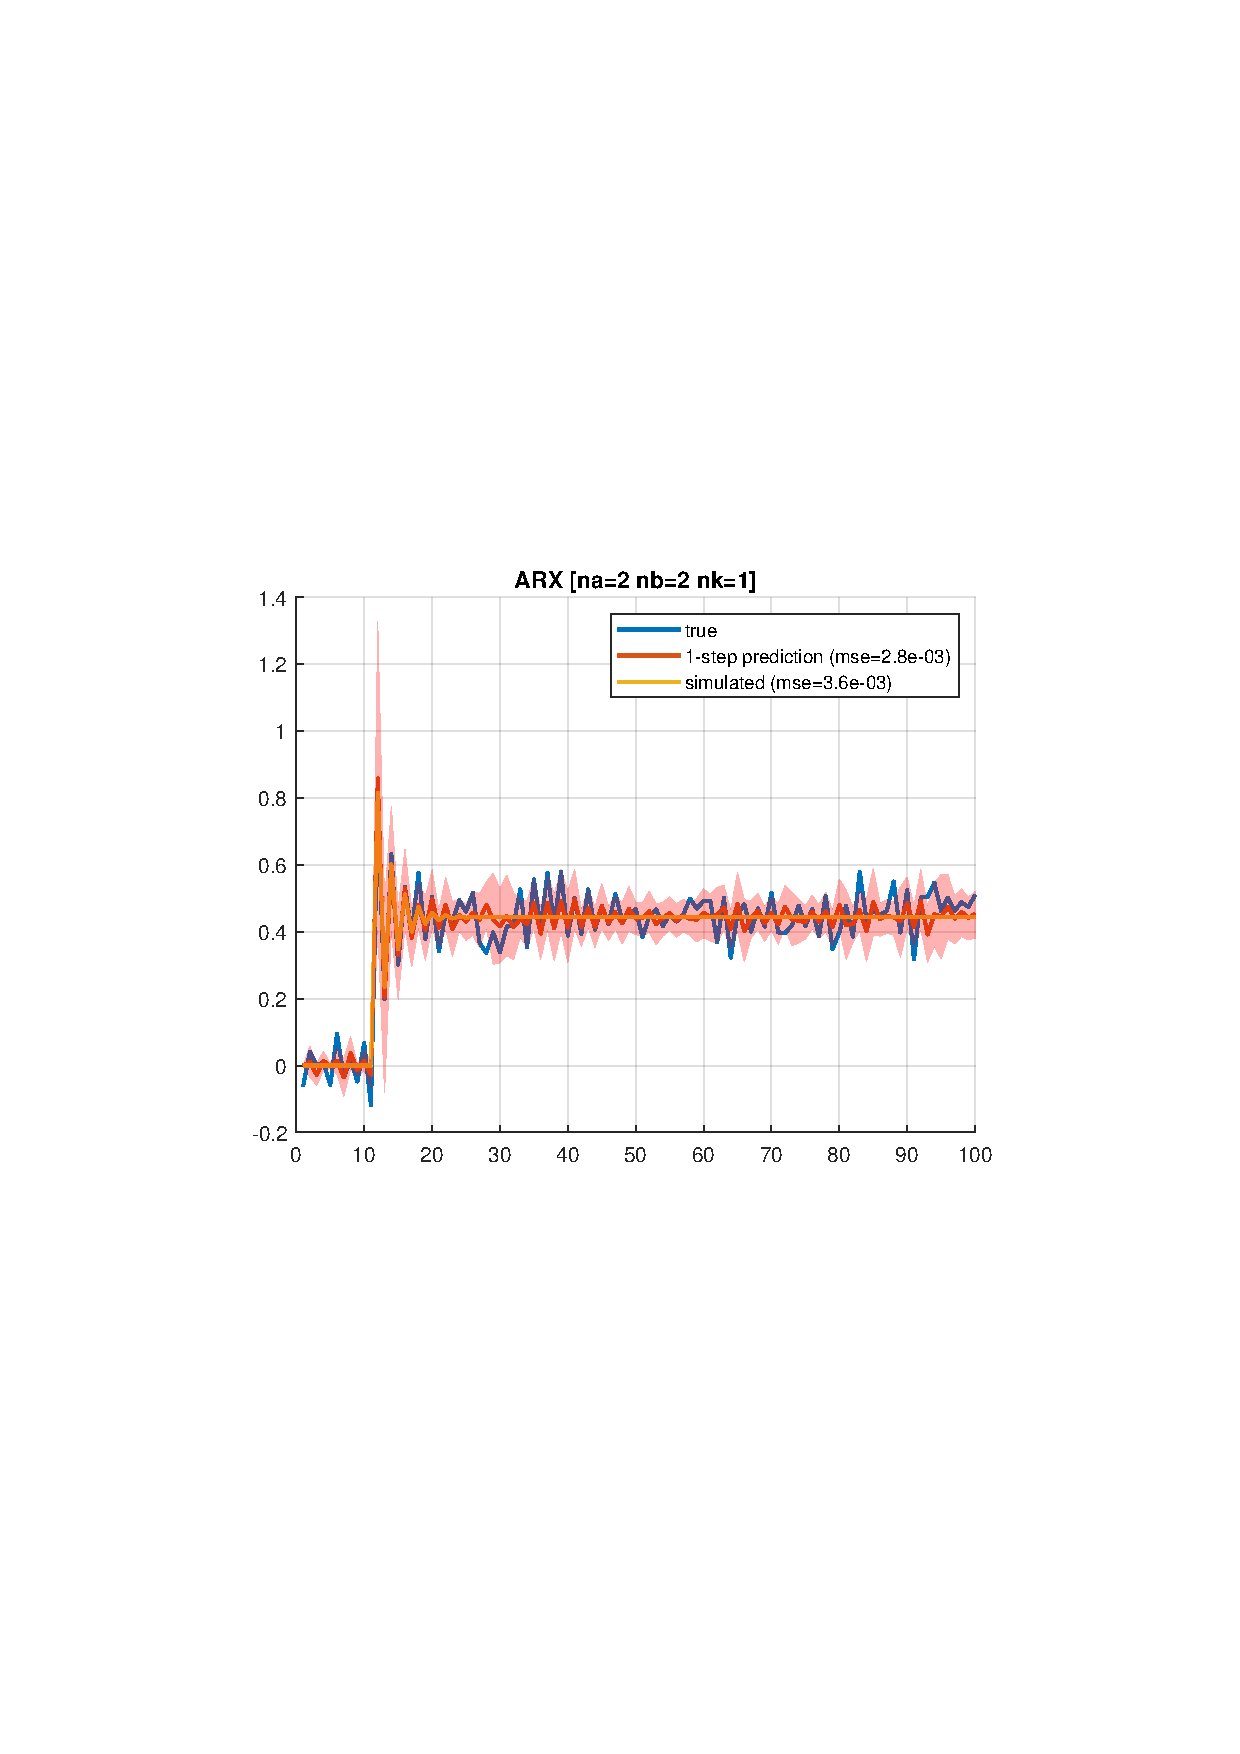
\includegraphics[trim= 10cm 8cm 10cm 8cm, scale=0.3]{figures/1d-horizon_1.pdf}
	\caption{Horizon 1}
	\label{fig:1d-horizon1}
\end{subfigure}
\begin{subfigure}{.30\textwidth}
	\centering
	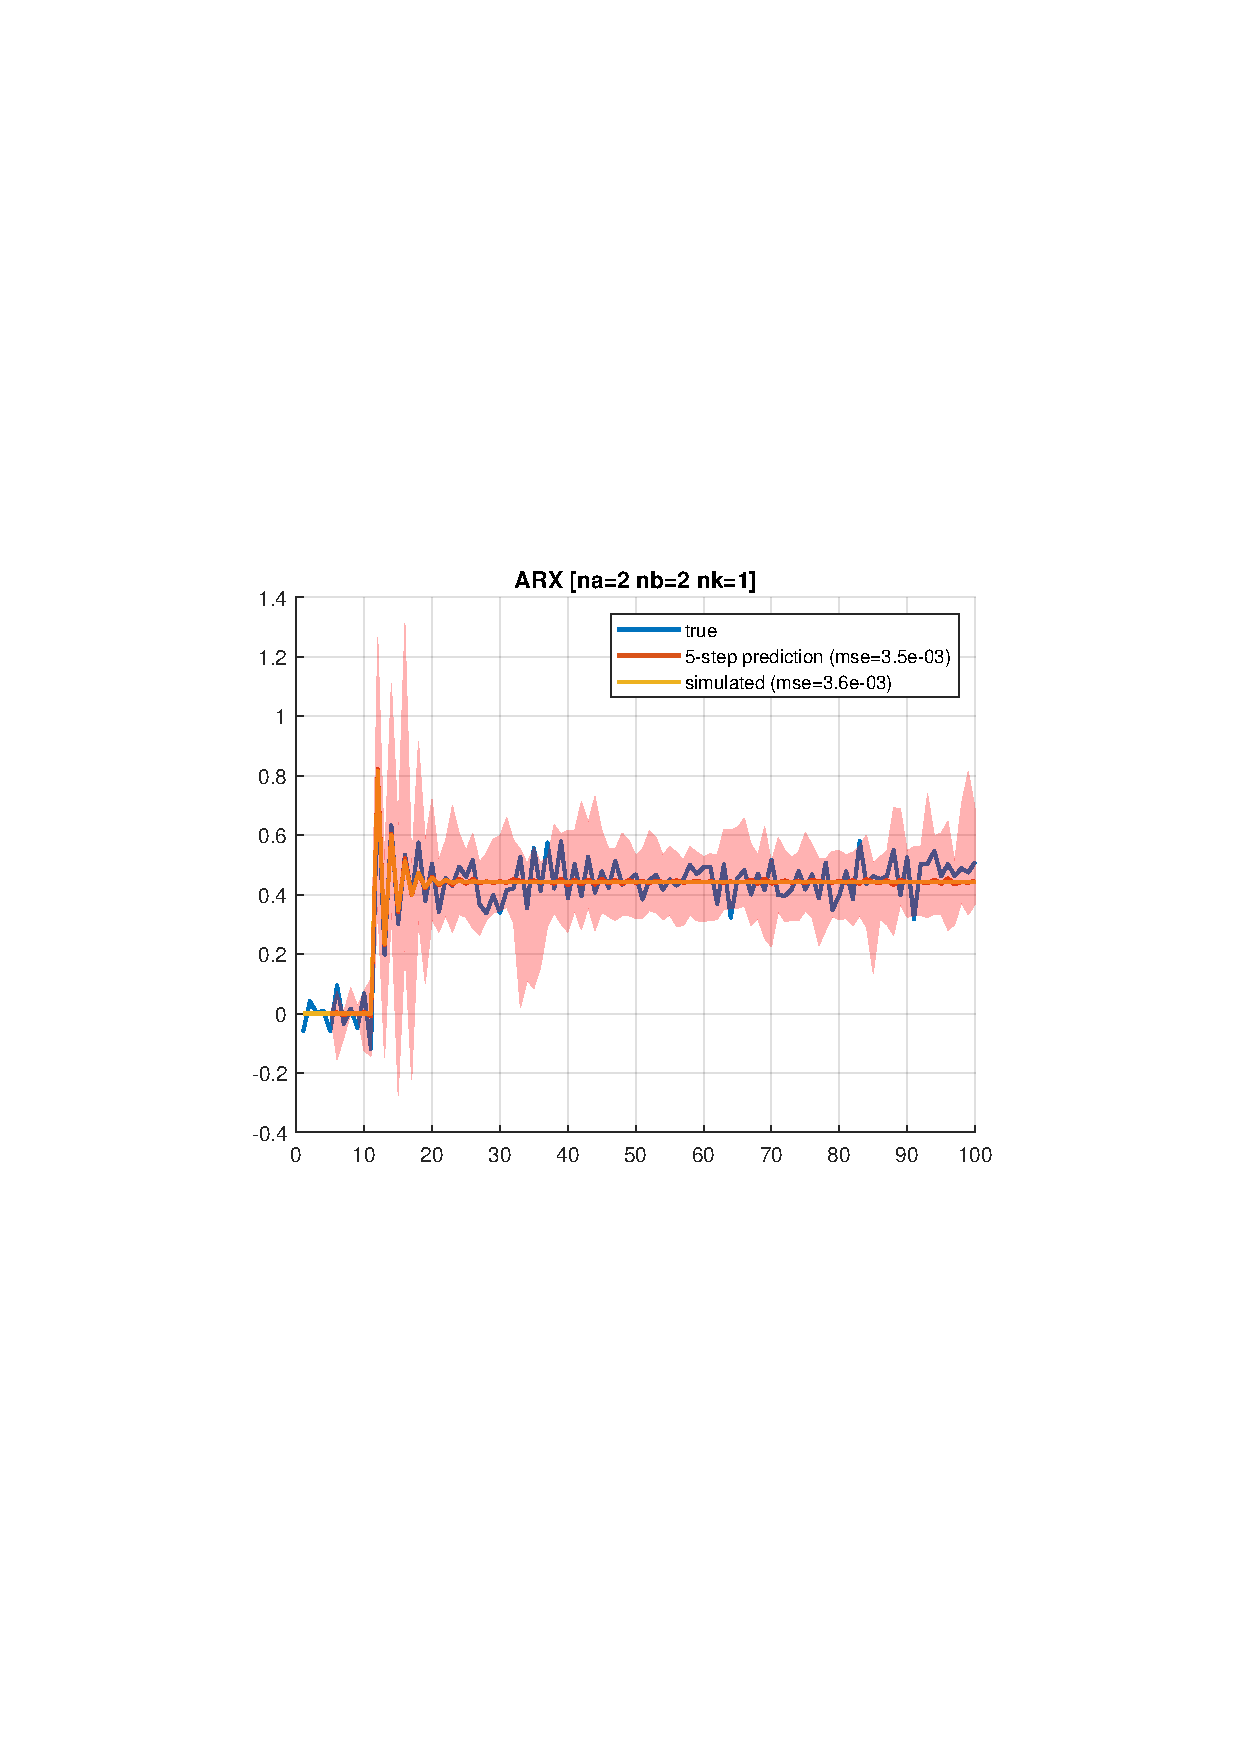
\includegraphics[trim= 10cm 8cm 10cm 8cm, scale=0.3]{figures/1d-horizon_5.pdf}
	\caption{Horizon 5}
	\label{fig:1d-horizon5}
\end{subfigure}
\begin{subfigure}{.30\textwidth}
	\centering
	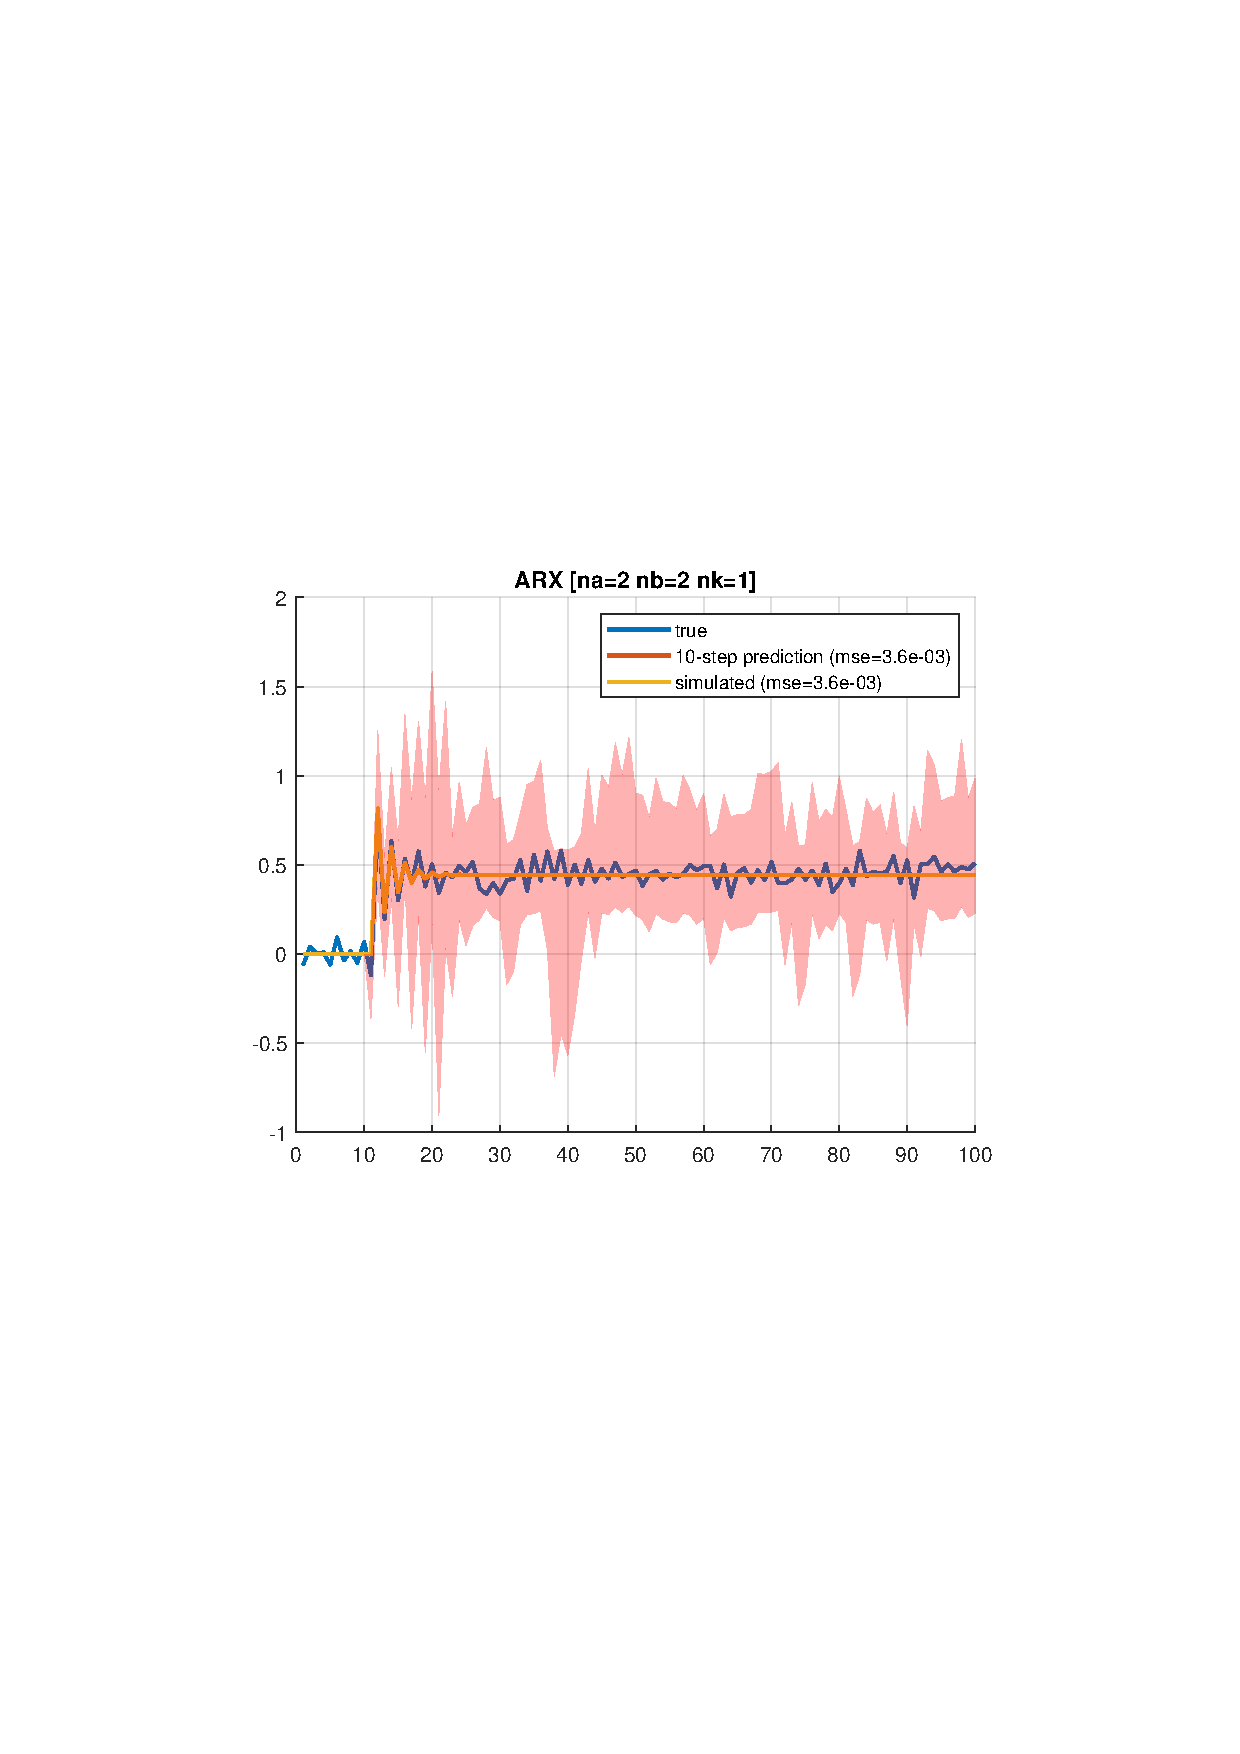
\includegraphics[trim= 10cm 8cm 10cm 8cm, scale=0.3]{figures/1d-horizon_10.pdf}
	\caption{Horizon 10}
	\label{fig:1d-horizon10}
\end{subfigure}
\caption{Some results using the implemented \emph{idcompare} function. It is clear that the model uncertainty is increasing for increasing horizons, which means that less data is allowed in the prediction step. The mse on validation data is also increasing as the horizon is increasing.}
\label{fig:1d}
\end{figure}

\section{OE estimator}

\subsection{(a) oefit}

\subsection{(b) id2tf}
No changes from ARX.

\subsection{(c) idpredict}
Changes necessary.

\subsection{(d) idsimulate}

\subsection{(e) idcompare}

\section{Identify two systems}

\end{document}
